\documentclass[tikz,border=0pt,11pt]{standalone}%
\usepackage{tikz-cd}
%\usepackage{ifthen}
\usetikzlibrary{arrows}
\begin{document}
%---------------------------Cascade-Correlation-------------------------------------------------------------%
% trim={<left> <lower> <right> <upper>}
%\adjustbox{trim=0pt 0pt 0pt 1.6cm,clip}{
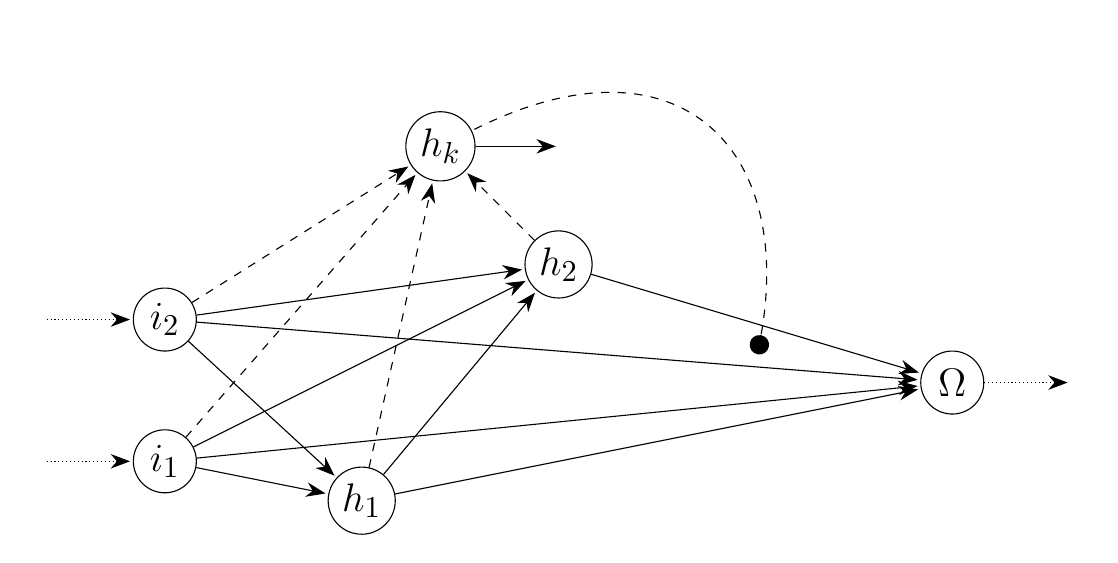
\begin{tikzpicture}[>=stealth', node distance=\layersep cm, shorten >=1pt]

        \def\layersep{2.5}          % vertikal distance between the layers
        \def\neuronsep{1.8}         % Horizontal distance between neurons
        \def\dlsize{2}              % distance between node and layer lable
        \def\inout{\layersep*.65}   % Size of in- and output-arrow
        \def\siz{.8}                % neuronsize
        \def\y{5}                   % Start of the most upper layer
        \tikzstyle{neuron}=[circle,draw=black,minimum size=\siz cm,inner sep=2pt]
        \tikzstyle{annot} = [text width=6em, text centered]
        \tikzset{fontscale/.style = {font={\fontsize{#1pt}{#1pt}\selectfont}}}

        % Draw the input layer nodes
        \node[neuron,fontscale=15] (Il-1) at (0,1*\neuronsep-\neuronsep) {$i_{1}$};
        \node[left of=Il-1, node distance=\inout cm] (Inl-1) {};
        \draw [->,arrows={-Stealth[length=7pt]},densely dotted] (Inl-1) edge (Il-1);

        \node[neuron,fontscale=15] (Il-2) at (0,2*\neuronsep-\neuronsep) {$i_{2}$};
        \node[left of=Il-2, node distance=\inout cm] (Inl-2) {};
        \draw [->,arrows={-Stealth[length=7pt]},densely dotted] (Inl-2) edge (Il-2);
        
        % Draw the hidden layer nodes
        \node[neuron] (Hl-1) at (1*\layersep,-.5) [fontscale=15] {$h_{1}$};
        \node[neuron] (Hl-2) at (2*\layersep,2.5) [fontscale=15] {$h_{2}$};
        
        % Draw the kandidate node
        \node[neuron] (Hl-3) at (1.4*\layersep,4) [fontscale=15] {$h_{k}$};
        \node[right of=Hl-3, node distance=\inout cm] (Hnl-3) {};
        \node[node distance=\inout cm] (Hnl-k) at (3*\layersep,1.2) {};
        \draw [->,arrows={-Stealth[length=7pt]}] (Hl-3) edge (Hnl-3);
        
        % Draw the output layer nodes
        \node[neuron] (Ol-1) at (4*\layersep,1) [fontscale=15] {$\Omega$};
        \node[node distance=\inout cm, right of=Ol-1] (Onl) {};
        \draw [->,arrows={-Stealth[length=7pt]},densely dotted] (Ol-1) edge (Onl);
        
        % Connect the neurons
        \foreach \name / \xn in {1,...,2}{
                \draw [->,arrows={-Stealth[length=7pt]},dashed] (Hl-\xn) edge (Hl-3);
                \foreach \source in {1,...,2}
                    \draw [->,arrows={-Stealth[length=7pt]}] (Il-\source) edge (Hl-\xn);
        }
        \draw [->,arrows={-Stealth[length=7pt]}] (Hl-1) edge (Hl-2);
        
        \foreach \source in {1,...,2}{
                \draw [->,arrows={-Stealth[length=7pt]},dashed] (Il-\source) edge (Hl-3);
                \draw [->,arrows={-Stealth[length=7pt]}] (Il-\source) edge (Ol-1);
                \draw [->,arrows={-Stealth[length=7pt]}] (Hl-\source) edge (Ol-1);
        }
        
        \draw[arrows={-Circle[length=7pt]}, shorten >=1pt, shorten <=1pt,dashed] (Hl-3) .. controls (6.5,5.5) and  (8,4) .. (Hnl-k);
        
        
\end{tikzpicture}
%}
\end{document}